Contracts that give one party the \textbf{(1)} \textit{right} to buy or sell a certain security, target risk better and information. \textbf{(2)} Allow us to learn incredibly granular levels of information. \textbf{(3)} target risks better and incredibly specific \textbf{(4)} Put information in a more targeted way. 

\begin{multicols}{2}
\subsection{Put Option}
The right to sell an asset for a certain price at a certain time in the future.
\subsection{Call Option}
The right to buy an asset for a certain price at a certain time in the future.
\subsection{Long Position}
The option buyer or holder pays a premium and receives the right to buy or sell an asset.
\subsection{Short Position}
The option seller or writer receives a premium and has the obligation to deliver or purchase an asset.
\subsection{Evaluate Options at Expiry}
\begin{itemize}
    \item $S_t$: Spot price, asset trading at time $t$.
    \item $X$: Strike or exercise price. 
    \item $T$: Strike or expiration date.
    \item $C_t$: Price of a call option.
    \item $P_t$: Price of a put option.
\end{itemize}

\end{multicols}

\begin{figure}[H]
    \centering 
    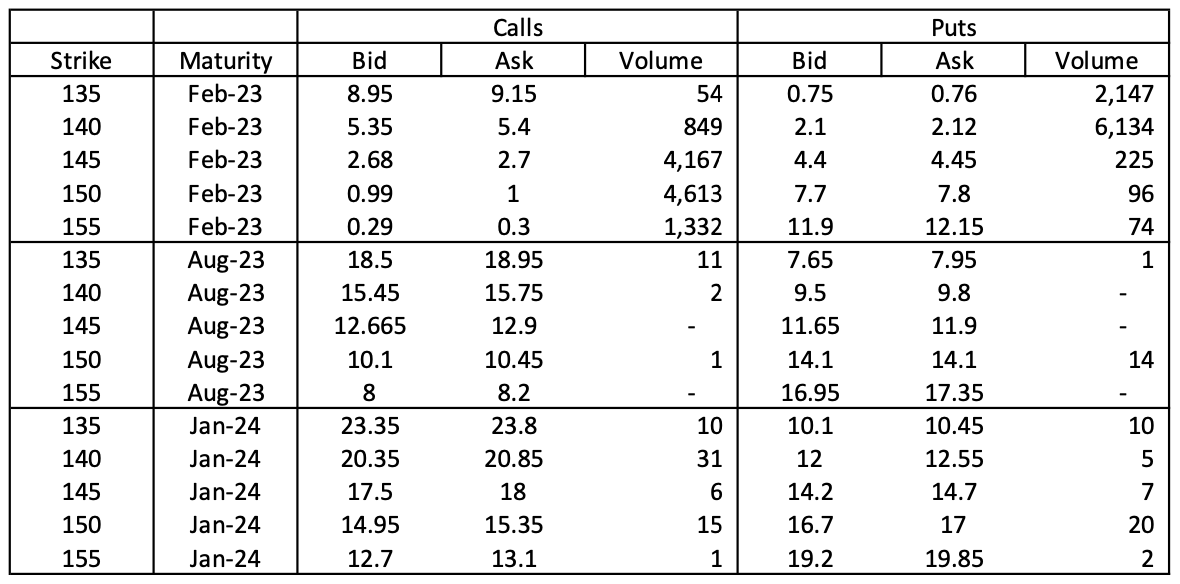
\includegraphics[width =0.7\textwidth]{Figure/option.png}
\end{figure}

\begin{multicols}{2}

From the Table above we can infer some information about the stock
\begin{itemize}
    \item The price of Call options decreases with increasing strike price, this is because people want to buy the stock at lower price instead of higher price, so I have to pay more for that right than the right to buy it at a more expensive price.
    \item The opposite is true for put options, where the right to sell at a lower price is less desirable
    \item For next-day expire option, if I know the price is not gonna change a lot between in one day for not very volatile stocks, and I know the right to buy this asset at say \$135 is \$9 today, it's probably gonna be \$9 tomorrow as well. Therefore, the value of the asset is most likely to be \$9 above \$135, which is around \$144 (or a range).
    \item options strictly has to be cheaper than the actual asset. It is also cheaper to buy an option if you think the price is going up.
\end{itemize}

A $\boxed{\textbf{Call option's value}}$ is:
\begin{gather*}
    C_T=\left\{
        \begin{array}{ll}
            \begin{split}
                S_T-X\hspace*{0.2cm}&\text{if}\hspace*{0.2cm}S_T>X\hspace*{0.2cm}\text{(in the money)}\\
                0\hspace*{0.6cm}&\text{if}\hspace*{0.2cm}S_T\leq X\hspace*{0.2cm}\text{(at/out of the money)}\\
            \end{split}
        \end{array}
        \right.
\end{gather*}
A $\boxed{\textbf{Put option's value}}$ is:
\begin{gather*}
    P_T=\left\{
        \begin{array}{ll}
            \begin{split}
                0\hspace*{0.6cm}&\text{if}\hspace*{0.2cm}S_T\geq X\hspace*{0.2cm}\text{(at/out of the money)}\\
                X-S_T\hspace*{0.2cm}&\text{if}\hspace*{0.2cm}S_T< X\hspace*{0.2cm}\text{(in the money)}\\
            \end{split}
        \end{array}
        \right.
\end{gather*}
\newpage

\end{multicols}

\begin{figure}[H]
    \centering 
    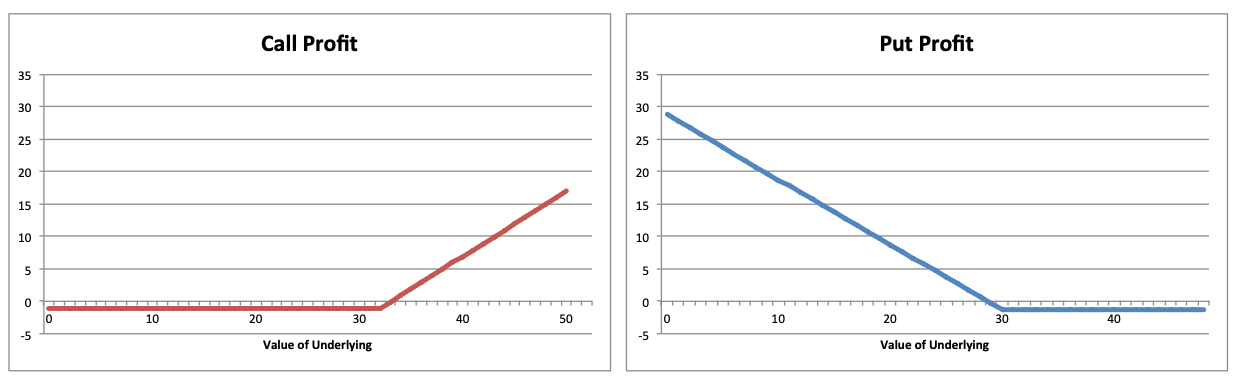
\includegraphics[width =0.7\textwidth]{Figure/long.png}
    \caption*{long option}
\end{figure}

\begin{figure}[H]
    \centering 
    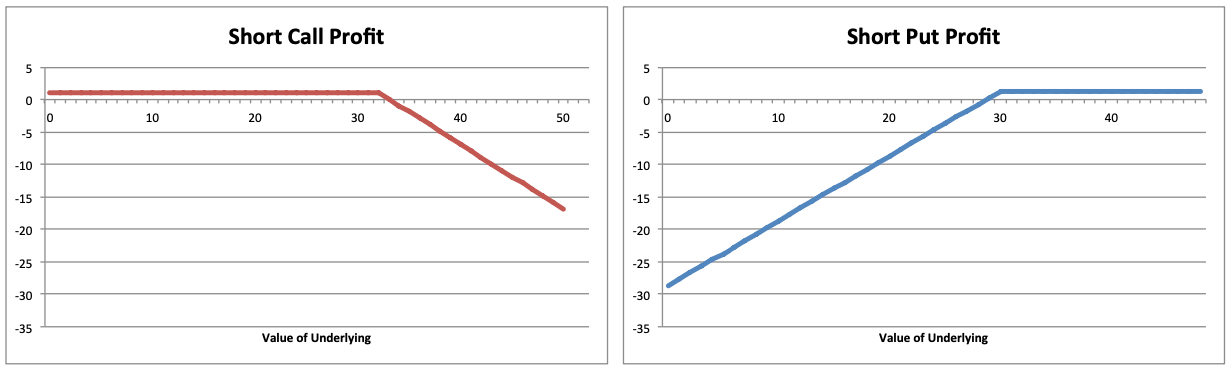
\includegraphics[width =0.7\textwidth]{Figure/short.png}
    \caption*{short option}
\end{figure}


\begin{multicols}{2}
\subsection{Option Strategies}
\subsubsection{Covered Calls}
\begin{itemize}
    \item Buy the stock at 30, and sell the call option. 
    \item if stock price goes up, earn money from stock but lose from selling the call option
    \item if stock price goes down, lose money from stock and earn a little for not exercising the sell option. 
    \item combination becomes a $\boxed{\textbf{short put option}}$
\end{itemize}
\begin{figure}[H]
    \centering 
    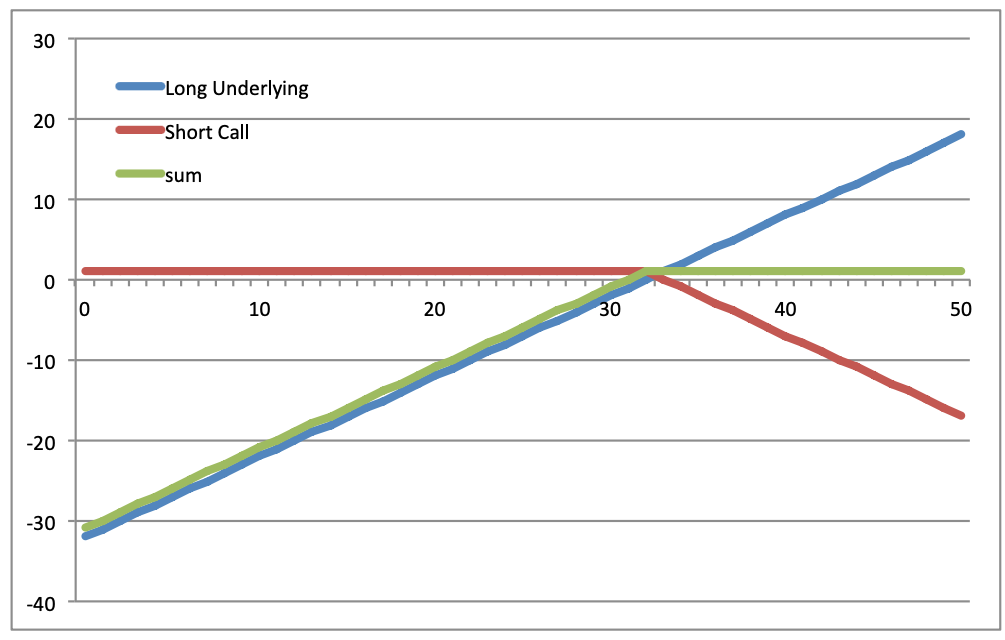
\includegraphics[width =0.45\textwidth]{Figure/cover_call.png}
\end{figure}

\subsubsection{Protected Put}
\begin{itemize}
    \item Buy the underlying, and buy a put option.
    \item The loss from the assets will be compensated by the profit made from the put option. 
    \item combination becomes a $\boxed{\textbf{call option}}$
\end{itemize}
\begin{figure}[H]
    \centering 
    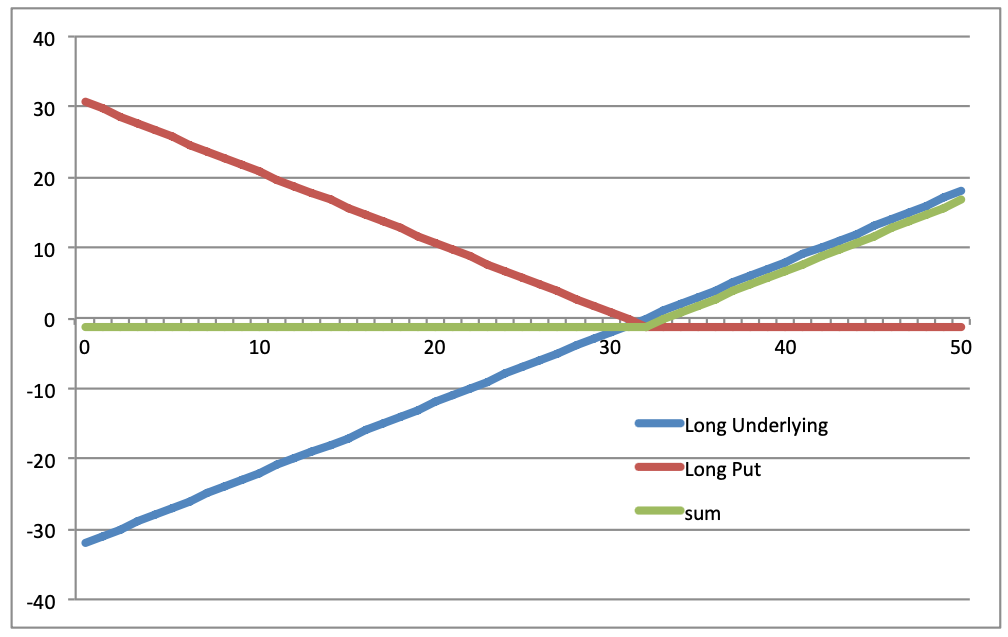
\includegraphics[width =0.45\textwidth]{Figure/protect_put.png}
\end{figure}
\textbf{covered calls} and \textbf{protected put} are ways to create the asset I want from assets I have. E.g. if I have the underlying asset and want to create a call option, I'll then buy a put, etc. 

\subsubsection{Bull Spread}
\begin{itemize}
    \item Buy a low-strike call option and sell a high-strike call option.
    \item given a fair amount of upside for less net losses. why?
    \item If you expect the asset to rise, but not that much, paying for the blue call option will be overpaying, therefore, the green line (sum) will be cheaper than the call option itself. 
    \item popular because it;s a managed cash flow, very low risk asset and fluctuations are small
\end{itemize}
\begin{figure}[H]
    \centering 
    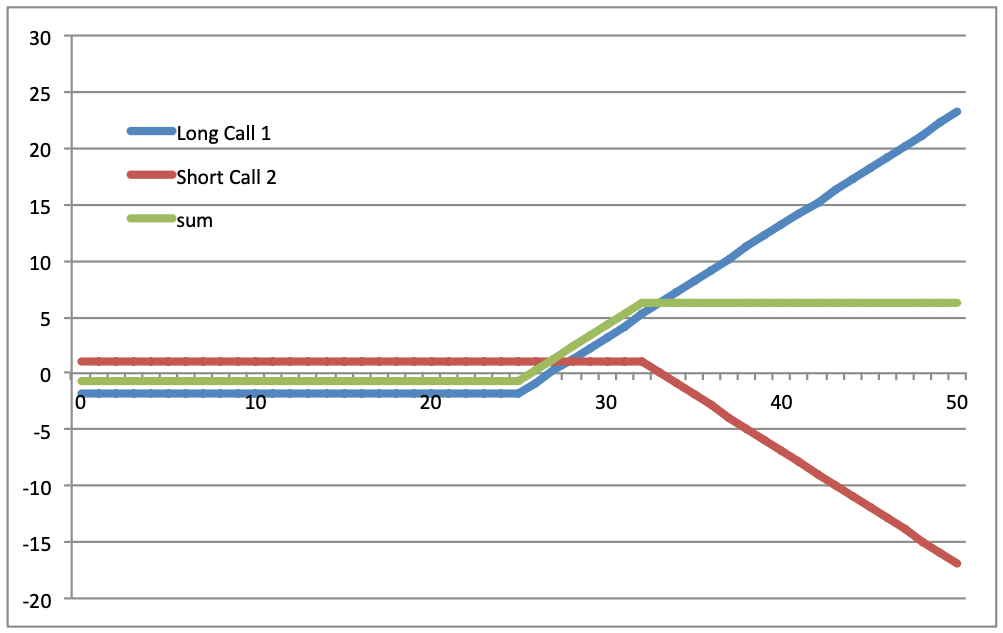
\includegraphics[width =0.45\textwidth]{Figure/bull.png}
\end{figure}

\subsubsection{Bear Spread}
\begin{itemize}
    \item Buy a high-strike call option and Sell a low-strike call option.
    \item flipped version of the bull Spread.
    \item gains and losses are capped, cheaper way to bet on downward price movements. 
\end{itemize}
\begin{figure}[H]
    \centering 
    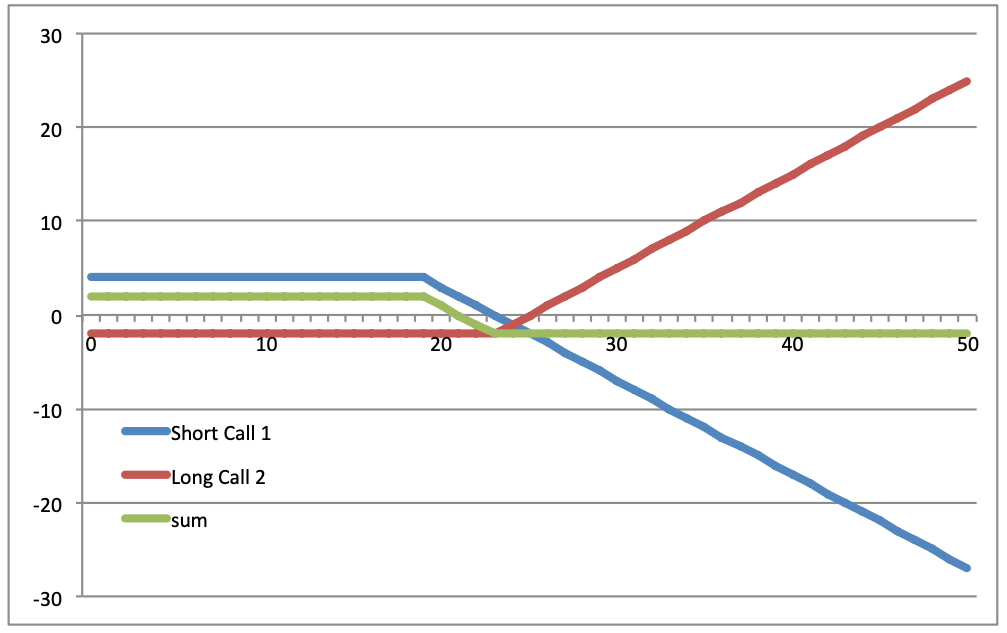
\includegraphics[width =0.45\textwidth]{Figure/bear.png}
\end{figure}

\subsubsection{Butterfly Spread}
\begin{itemize}
    \item Buy a low strike bull spread and sell a high strike bull spread.
    \item Call($X_1$)-Call($X_2$) - (Call($X_2$)-Call($X_3$)) = Call($X_1$)-2Call($X_2$)+Call(X$X_3$)
    \item An extremely target bet, therefore, the price of this asset will be very informative about how likely the market thinks the final value of the underlying is gonna stay in that region.
    \item can use this spread to infer the underlying volatility.
\end{itemize}
\begin{figure}[H]
    \centering 
    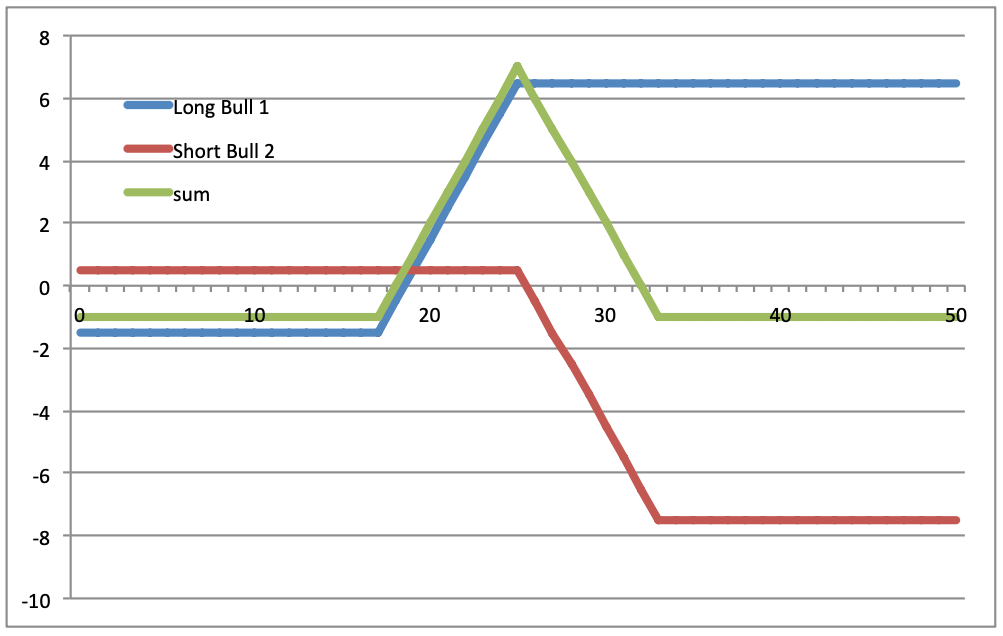
\includegraphics[width =0.45\textwidth]{Figure/butter.png}
\end{figure}

\subsubsection{Straddles/strangles}
\begin{itemize}
    \item Buy a put option and a call option at the same (different) strikes
    \item Bets purely on the volatility of the asset
    \item for straddle, you make money as long as the price changes. 
    \item for strangle, make money with minimum threshold. 
\end{itemize}
\begin{figure}[H]
    \centering 
    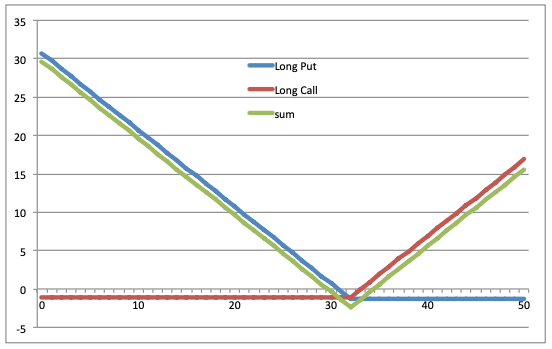
\includegraphics[width =0.45\textwidth]{Figure/straddle.png}
    \caption*{straddle}
\end{figure}

\begin{figure}[H]
    \centering 
    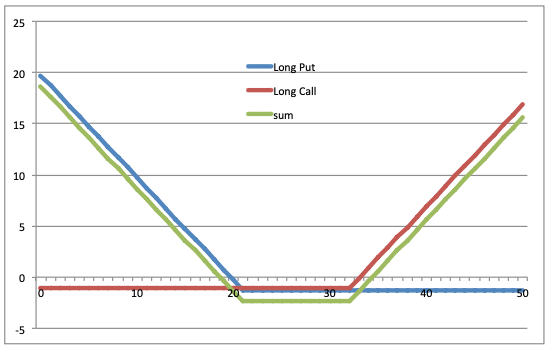
\includegraphics[width =0.45\textwidth]{Figure/strangle.png}
    \caption*{strangle}
\end{figure}
\subsubsection{Strips/straps}
\begin{itemize}
    \item Strips is a straddle with an additional put 
    \item strips makes money as long as the price moves, but make more if the price moves down 
    \item Strap is a straddle with an addition call
    \item straps makes money as long as the price moves, but make more if the price moves up
\end{itemize}

\begin{figure}[H]
    \centering 
    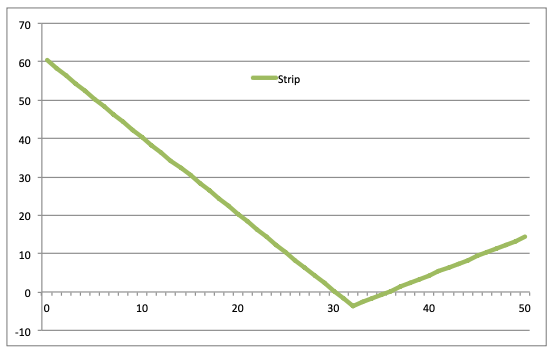
\includegraphics[width =0.28\textwidth]{Figure/strip.png}
\end{figure}
\vspace*{-0.9cm}
\begin{figure}[H]
    \centering 
    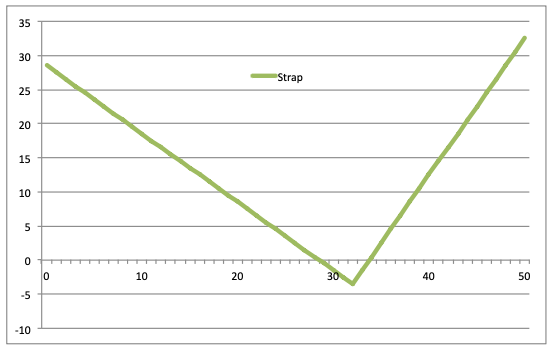
\includegraphics[width =0.28\textwidth]{Figure/strap.png}
\end{figure}

\subsection{Put-Call Parity}
\begin{itemize}
    \item (1) If I buy a call and sell a put option at the same strike price. 
    \item (2) And I also buy the stock 
    \item (3) Also lend the present value of the strike price. 
    \item Put-Call parity states that the blue line plus the red line plus the purple line should equal to the green line. 
    \begin{figure}[H]
        \centering 
        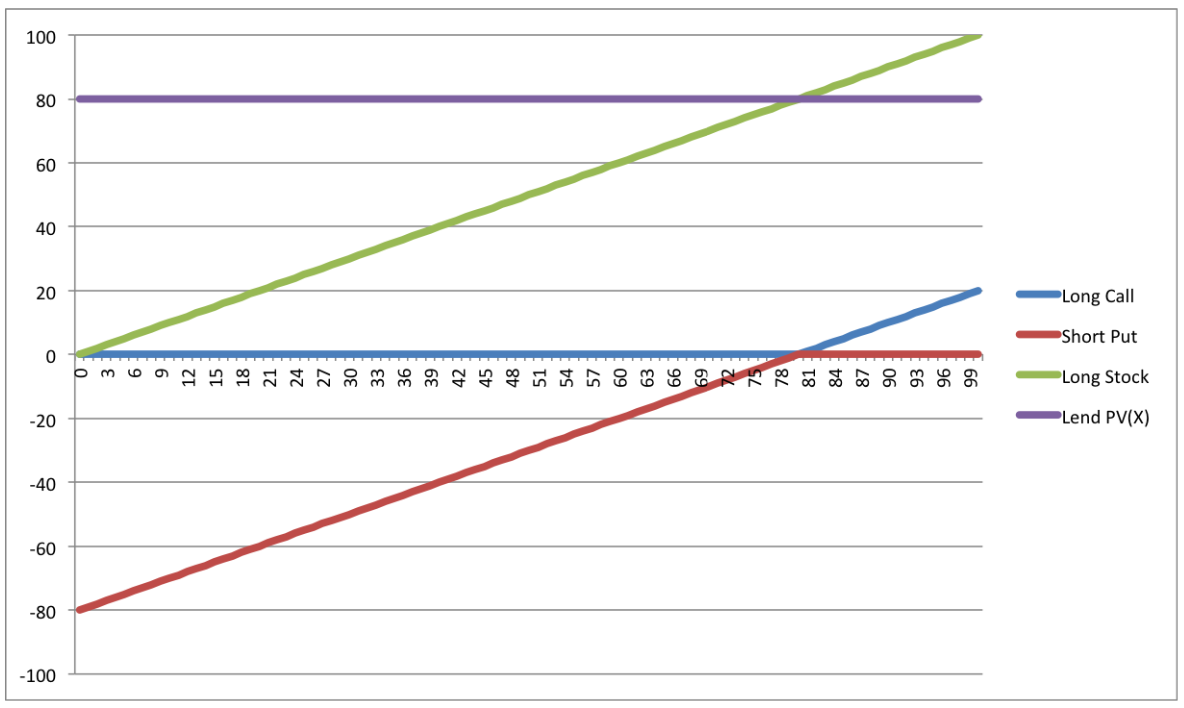
\includegraphics[width =0.35\textwidth]{Figure/parity.png}
    \end{figure}
\end{itemize}
\begin{gather*}
    \boxed{C(K,T)-P(K,T) = S_0-e^{-rT}K}
\end{gather*}
Where $C$ is the price of a call, $P$ is the price of a put, $T$ is the time to expiry, $K$ is the strike, $S_0$ is the spot price of the underlying, and $r$ is the risk-free rate. 
\begin{table}[H]
    \begin{tabular}{c|c|c|c}
    Action & Today & $S_T<$X & $S_T>$X \\ \hline
    Buy a call & -C & $S_T$-X & 0 \\ 
    write a put & +P & 0 & $S_T$-X \\ 
    Lend PV(X) at R & -e$^{rT}$X & X & X \\
    Net cashflow & $\underbrace{P-C-e^{rT}X}_{S_0}$ & $S_T$ & $S_T$ \\
    \end{tabular}
\end{table}
\vspace*{-0.5cm}
By buying a call, selling a put, and lend the present value of the strike, I ended up with a portfolio $S_T$, which implies that I ended up owning the stock, or owning the cash equivalent of the stock no matter the stock does well or bad. So another way to \textit{own} a stock is to \textit{buy} the stock. Thus, this portfolio perfectly replicates the payoffs of owning this stock.

\subsection{Option Pricing}
\subsubsection{Risk-Neutral Probability Distribution}
Say I offer a lottery to bet on a fair coin toss ($P(H)=P(T)=0.5$), if it lands on head I'll give you \$100, and nothing if it lands on tails. Say the certainty equivalent is \$30 (the price of the lottery is \$30)\footnote{The certainty equivalent cash flow is the risk-free cash flow that an investor or manager considers equal to a different expected cash flow which is higher, but also riskier. It is closely related to the concept of \textbf{risk premium} or the amount of additional return an investor requires to choose a risky investment over a safer investment}, the probability of hands is then $Q(H)=30/100 = 0.3\%$, and the probability of tails is then $Q(T) = 70\%$. Why is that the $Q(H)<P(H)$?? Why are we not willing to pay \$50 for the lottery??\par 

Because the lottery is \textbf{risky}, we won't pay the actuarially price (\$50), therefore, the difference between the actuarially price and the price we are willing to pay (\$30) is the \underline{risk premium}. Thus, the distribution extract by looking at the price will be skewed because the probability assigned to heads is lower than the truth when riskiness is involved. People on average tends to be risk averse that they won't pay the actuarially fair price.\par 

\textbf{Good states of the world will be undervalued (0.3), bad states will be overvalued (0.7)}. This is how risk aversion shows up in prices. The Risk-Neutral Distribution (Q)\footnote{Under the assumption of risk neutrality, investors do not require a higher expected return to compensate them for taking on more risk, and they do not penalize investments with higher risk. Instead, they only care about the expected return of the investment, which is the weighted average of the possible outcomes of the investment, where each outcome is weighted by its probability.} tells us about the physical probability (P) but also with risk aversion, and it's hard to separate these two. 

\subsubsection{How to get Q distribution}
Consider three call options with the same maturity but different strike price:
\begin{itemize}
    \item Call C(14) @ \underline{2.21}
    \item Call C(15) @ \underline{1.56}
    \item Call C(16) @ \underline{1.05}
\end{itemize}
\begin{figure}[H]
    \centering 
    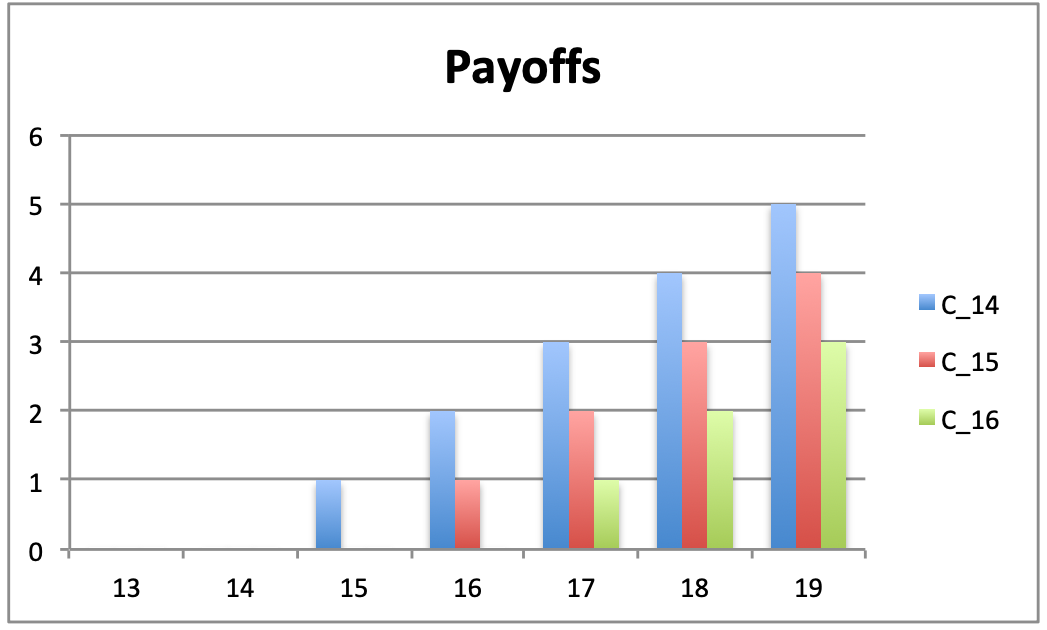
\includegraphics[width =0.28\textwidth]{Figure/Q_call.png}
\end{figure}
And then we construct a bull spread with these call options (Bull spread: buy low strike call, sell high strike call) 
\begin{itemize}
    \item Bull(14,15) @ (2.21-1.56 = \underline{0.65})
    \item Bull(15,16) @ (1.56-1.05 = \underline{0.51})
\end{itemize}
\begin{figure}[H]
    \centering 
    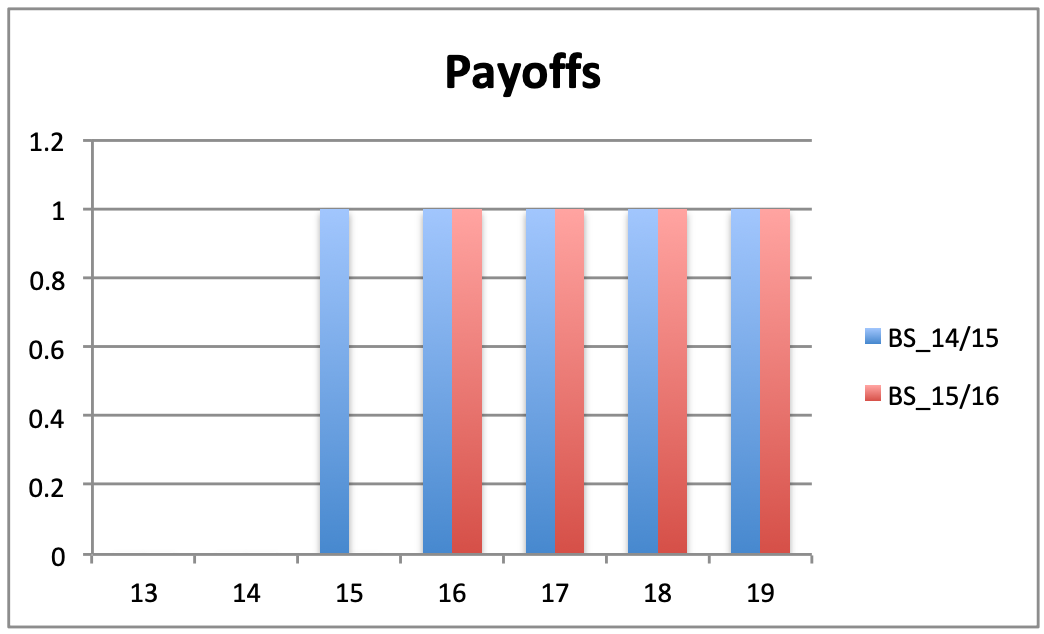
\includegraphics[width =0.28\textwidth]{Figure/Q_bull.png}
\end{figure}
And finally, if we construct a butterfly spread (Buy low strike bull, sell high strike bull). 
\begin{itemize}
    \item Butterfly(14,15,16) @ (0.65-0.51 = \underline{0.14})
\end{itemize}
\begin{figure}[H]
    \centering 
    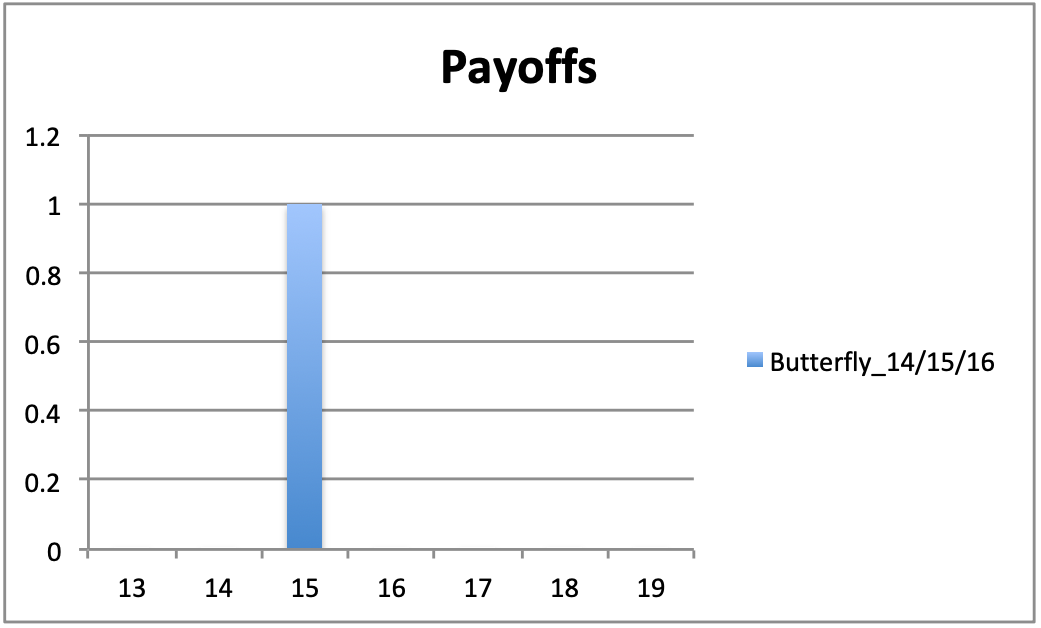
\includegraphics[width =0.28\textwidth]{Figure/Q_butter.png}
\end{figure}
This particular butterfly spread price Arrow-Debreu Securities, where if one particular state of the world happens you get \$1 and \$0 if any other state of the world happens.\par

what does the price \underline{\textbf{0.14}} tells us? 0.14 is the \textbf{risk-weighted probability} that includes the risk aversion of people, also reflects the aggregate beliefs. From a mathematical sense, we can also express the above as (per dollar price):
\begin{gather*}
    \begin{split}
        &\text{Bull spread} = \frac{C(X+\varepsilon)-C(X)}{X+\varepsilon-X} = \boxed{C^\prime(X)}\\[0.2cm]
        &\text{Butterfly} = \frac{\text{Bull}(X+2,X+1)-\text{Bull}(X+1,X)}{X+1-X}=\boxed{C^{\prime\prime}(X)}
    \end{split}
\end{gather*}
This shows that we can use options prices to extract risk-neutral probabilities. We can use this probability distribution to account for the volatility of the asset (option), by calculating the standard deviation of the resulting distribution by extracting forward-looking expectation from prices. Because options are stackable, you can create extremely targeted bets, which give you extremely specific pieces of information. This probability includes risk aversion. 

\subsubsection{Option Pricing}
I have a stock ($S_0=100$), A bond ($B_0=100$) with $R_f=2\%$, and I want to replicate a call option $C$ with strike price $K$. 
\begin{figure}[H]
    \centering 
    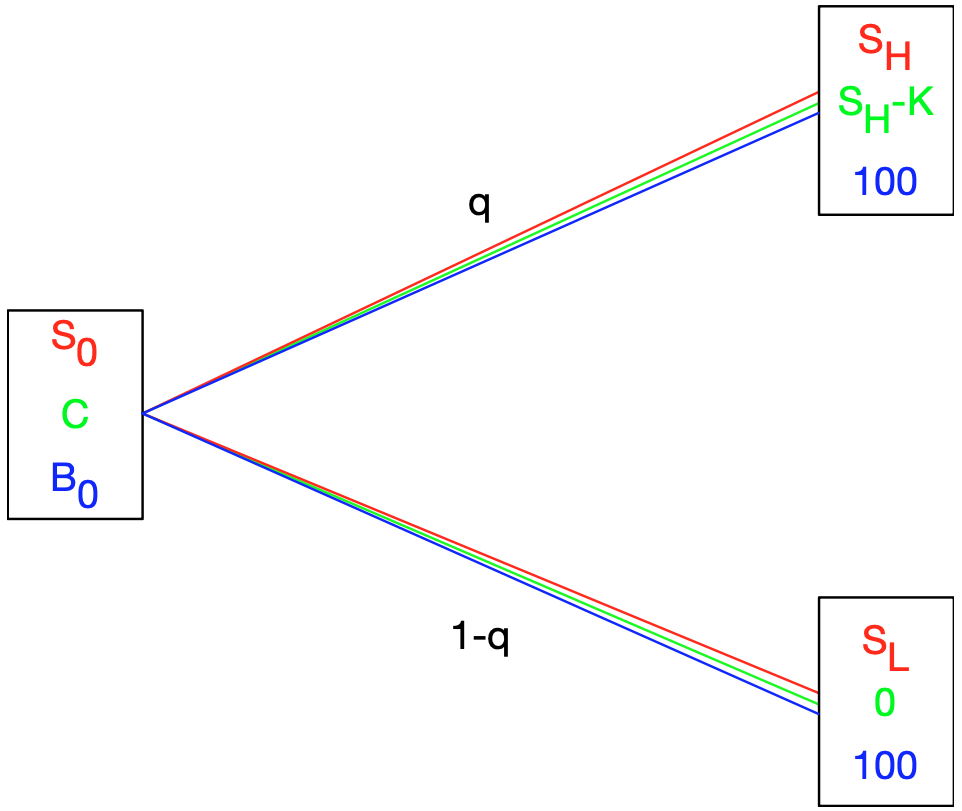
\includegraphics[width =0.2\textwidth]{Figure/tree.png}
\end{figure}
If I try to replicate the payoffs of the call option by buying $\Delta$ amount of stock $S_0$ and $X$ unit of bond $B$. Assume that for high scenarios, the stock $S_H = 110$, and at low times, the stock $S_L = 90$, whereas the bond pays 100 no matter what. Therefore, the call at maturity for high is \$10, and \$0 at low. 
\begin{gather*}
    \Delta110+X100=10\\
    \Delta90+X100=0\\
    \therefore\hspace*{0.2cm}\Delta = 0.5,\hspace*{0.2cm}X=-0.45
\end{gather*}
If i can replicate the payoff of the call option, the price of the replicating portfolio must equal to the price of the call option.
\begin{gather*}
    \Delta\cdot S_0 + X\cdot B_0 = 0.5\cdot100-0.45\cdot\frac{100}{1.02} = 5.88
\end{gather*}

If the stock price change by 1 dollar, the value of the call option change by $\Delta$ dollars, sensitivity of the option price to the underlying asset, which is the beta.
$X$ tells you the sensitivity of the call option price effectively to the risk-free rate or to the bond price.

\end{multicols}
